%%%%%%%%%%%%%%%%%%%%%%%%%%%%%%%%%%%%%%%%%
% Short Sectioned Assignment
% LaTeX Template
% Version 1.0 (5/5/12)
%
% This template has been downloaded from:
% http://www.LaTeXTemplates.com
%
% Original author:
% Frits Wenneker (http://www.howtotex.com)
%
% License:
% CC BY-NC-SA 3.0 (http://creativecommons.org/licenses/by-nc-sa/3.0/)
%
%%%%%%%%%%%%%%%%%%%%%%%%%%%%%%%%%%%%%%%%%

%----------------------------------------------------------------------------------------
%	PACKAGES AND OTHER DOCUMENT CONFIGURATIONS
%----------------------------------------------------------------------------------------

\documentclass[paper=a4, fontsize=11pt]{scrartcl} % A4 paper and 11pt font size

\usepackage[T1]{fontenc} % Use 8-bit encoding that has 256 glyphs
\usepackage{fourier} % Use the Adobe Utopia font for the document - comment this line to return to the LaTeX default
\usepackage[english]{babel} % English language/hyphenation
\usepackage{amsmath,amsfonts,amsthm, amssymb} % Math packages
\usepackage{slashed}

\usepackage{graphicx}
\usepackage{multicol}
\usepackage{enumitem}
\usepackage{caption}
\usepackage{esint}

\usepackage{listings}
\usepackage{color}

\definecolor{dkgreen}{rgb}{0,0.6,0}
\definecolor{gray}{rgb}{0.5,0.5,0.5}
\definecolor{mauve}{rgb}{0.58,0,0.82}

\lstset{frame=tb,
  language=C,
  aboveskip=3mm,
  belowskip=3mm,
  showstringspaces=false,
  columns=flexible,
  basicstyle={\small\ttfamily},
  numbers=none,
  numberstyle=\tiny\color{gray},
  keywordstyle=\color{blue},
  commentstyle=\color{dkgreen},
  stringstyle=\color{mauve},
  breaklines=true,
  breakatwhitespace=true
  tabsize=3
}

\usepackage{lipsum} % Used for inserting dummy 'Lorem ipsum' text into the template

\usepackage{sectsty} % Allows customizing section commands
\allsectionsfont{\centering \normalfont\scshape} % Make all sections centered, the default font and small caps

\usepackage{abstract}
\renewcommand{\abstractnamefont}{\normalfont\Large}
\renewcommand{\abstracttextfont}{\normalfont}

\usepackage{fancyhdr} % Custom headers and footers
\pagestyle{fancyplain} % Makes all pages in the document conform to the custom headers and footers
\fancyhead{} % No page header - if you want one, create it in the same way as the footers below
\fancyfoot[L]{} % Empty left footer
\fancyfoot[C]{} % Empty center footer
\fancyfoot[R]{\thepage} % Page numbering for right footer
\renewcommand{\headrulewidth}{0pt} % Remove header underlines
\renewcommand{\footrulewidth}{0pt} % Remove footer underlines
\setlength{\headheight}{13.6pt} % Customize the height of the header

\numberwithin{equation}{section} % Number equations within sections (i.e. 1.1, 1.2, 2.1, 2.2 instead of 1, 2, 3, 4)
\numberwithin{figure}{section} % Number figures within sections (i.e. 1.1, 1.2, 2.1, 2.2 instead of 1, 2, 3, 4)
\numberwithin{table}{section} % Number tables within sections (i.e. 1.1, 1.2, 2.1, 2.2 instead of 1, 2, 3, 4)

%\setlength\parindent{0pt}  Removes all indentation from paragraphs - comment this line for an assignment with lots of text

%Average
\newcommand{\average}[1]{\ensuremath{\left\langle #1 \right\rangle}}
%Parenthesis 
\newcommand{\parentheses}[1]{\ensuremath{\left( #1 \right)}}
%Commutator
\newcommand{\commutator}[1]{\ensuremath{\left[ #1 \right]}}
%Anti-commutator
\newcommand{\anticommutator}[1]{\ensuremath{\left\lbrace #1 \right\rbrace}}
%QED
\newcommand{\QED}{\begin{flushright}\textit{Q.E.D.}\end{flushright}}
%Split
\newcommand{\spliteq}[1]{\begin{split} #1 \end{split}}
%----------------------------------------------------------------------------------------
%	TITLE SECTION
%----------------------------------------------------------------------------------------

\newcommand{\horrule}[1]{\rule{\linewidth}{#1}} % Create horizontal rule command with 1 argument of height

\title{
\vspace{-2.5cm}
\begin{center}

\includegraphics[width=2.5cm]{logo-kth.png}\\[-1mm]
\hspace{-3mm}
\end{center}
\normalfont \normalsize
\textsc{Theoretical Physics} \\ [25pt] % Your university, school and/or department name(s)
\horrule{0.5pt} \\[0.4cm] % Thin top horizontal rule
\huge GPU Acceleration of the Ising Spin Glass \\ % The assignment title
\Large Advanced Computational Physics\\ % Course name
\Large SI2531, Fall 2014\\ % Course code and Semester
\Large Supervisor: Prof. Mats Wallin \\ %Supervisor
\horrule{2pt} \\[0.5cm] % Thick bottom horizontal rule
}

\author{Jens Wir\'{e}n \\
Farhad Kimanos \\
Stefan Fleischmann \\
\normalsize jenswir@kth.se \\
\normalsize kimanos@kth.se \\
\normalsize sfle@kth.se} % Your name

\date{\normalsize\today} % Today's date or a custom date

\begin{document}

\maketitle % Print the title

%----------------------------------------------------------------------------------------

\begin{abstract}
We study the stiffness exponent $\theta$ of a two and three dimensional Ising spin glass model with Gaussian couplings on a square lattice. The disordered ground state and the domain wall energy $\Delta E$ is obtained by quenching the system from $T=\infty$ to $T=0 K$ for various system sizes and $\theta$ is calculated from the scaling anzats $\Delta E \thicksim L^\theta$ where $L$ is the system size. The results obtained agree well with the known values, $\theta_{2D}=-0.289$ and $\theta_{3D}=0.225$, for two and three dimensions respectively.

The method used is an optimized GPU-accelerated double checker board algorithm written in Compute Unified Device Architecture (CUDA) language and run on a Nvidia Tesla C2070 graphics card. The algorithm is benchmarked and computation times are displayed and commented on.
\end{abstract}

\pagebreak

\tableofcontents

\section{Introduction}

The goal of this project is to examine an Ising spin glass model with Gaussian couplings in two and three dimensions to determine the stiffness exponent $\theta$ using a GPU-accelerated algorithm. 

The paper is outlined as follows. Starting of in Section \ref{sec:theory} the Ising model, frustration and spin glasses will introduced, explained and previous work on spin glasses will be mentioned. Section \ref{sec:method} contains a detailed overview of GPU architecture, the implementation using CUDA and finally optimization. Results from the simulations as well as benchmarking statistics is displayed in Section \ref{sec:results} and are discussed in the final Section \ref{sec:discussion}.

\section{Theory}
\label{sec:theory}

\subsection{The Ising Model}

The Ising model is one of physics most studied models concerning spin systems. It is both easy to define yet extremely rich in it is behaviour. With small variations the Ising model can describe many interesting systems from the common ferromagnet to the exotic spin glass systems to be examined.

The Ising model is defined by the Hamiltonian

\begin{equation}
H = -J \sum\limits_{\left\langle i,j \right\rangle} S_{i} S_{j} -h \sum\limits_{i} S_{i}
\end{equation}
where $S_{i} = \pm 1$ is a spin degree of freedom on lattice site $i$, $\left< i,j \right> $ means nearest neighbour summation, $h$ is an applied magnetic field and $J$ is a coupling
constant. When $J$ is set to $J=+1$ this represents a ferromagnetic and when $J=-1$ an antiferromagnetic. We will only consider the case with no external field, i.e. $h=0$.

\subsection{Frustration}
The 2D Ising model defined on a square lattice is the only one with an analytical solution apart from the 1D Ising chain. Even thou this set up is the easiest in the two-dimensional case the exact solution, first solved by Onsager, is famously complicated\cite{onsager}. 

When using ferromagnetic couplings the ground state of this model is simply all spins oriented in the same direction, either up or down. In the antiferromagnetic case it is a checker board pattern of spin up and down. In both these cases the ground state is  two-fold degenerate since inverting all spins simultaneously does not affect the ground state. If we define the 2D Ising model on a triangular lattice with ferromagnetic couplings the ground state is still all spin up or down. The antiferromagnetic case however is quite different.

Consider the triangular unit cell and attempt to minimize the energy. Let the top position of the triangle be the first spin, one can orientate this arbitrarily but lets choose up for now without loss of generality. Let the bottom left of the triangle be the second spin and we will now choose this to be down in order to minimize the energy with respect to the first spin. But how is one suppose to orientate the third and final spin located in the bottom right? 

If one chooses this to be spin up we minimize the energy with respect to the second spin but maximize with respect to the first one. If we instead choose spin down the situation is reversed. We can never satisfy the other two spins simultaneously. This means that the ground state of the system will never be as low as for the square lattice or ferromagnetic case. Furthermore the ground state is highly degenerate since there is no unique way to reach it. This phenomenon is known as \emph{geometric frustration} and is illustrated in Figure \ref{fig:frustration}.

\begin{figure}
\centering
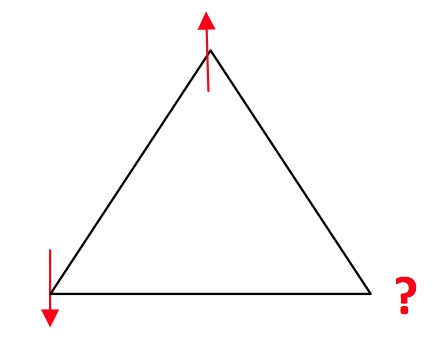
\includegraphics[scale=0.5]{images/frustration.jpg}
\caption{In the antiferromagnetic 2D Ising model on a triangular lattice there is no way one can orient the spins to minimize all interactions simultaneously.}
\label{fig:frustration}
\end{figure}

\subsection{The Ising Spin Glass}
In the previous section we concluded by introducing the concept of frustration through geometric frustration on a triangular lattice. There are however other ways to create frustrated systems and one of them is to introduce a new Hamiltonian

\begin{equation}
H=\sum\limits_{\left\langle i,j \right\rangle} J_{ij} S_{i} S_{j}
\end{equation}
where the coupling constants $J_{ij}$ now is a Gaussian random variable with zero mean and variance one. This Hamiltonian describes a class of disordered systems and we will focus on a subgroup of these called \emph{spin glasses} (SGs). What is special about SGs is the fact that they have a finite temperature disordered ground state. This means that below a critical temperature $T_c$ the disordered system will "freeze" with the spins in random positions determined by the particular set of couplings used. However, depending on the dimension of the lattice used there is a critical dimension below which there exists no finite temperature glass phase\cite{almeida}.

The main objective when examining disordered system is often to determine the critical exponents and we will concern ourselves with one of these, namely the \emph{stiffness exponent} $\theta$. This can be obtained through the scaling anzats

\begin{equation}
\Delta E \thicksim L^\theta
\label{eq:scaling}
\end{equation}
where $L$ is the system size and $\Delta E$ is the cost of a domain wall. We will use the tried and true P-AP method\cite{hartmann}\cite{carter} to calculate $\Delta E$ which can outlined as follows:

\begin{enumerate}
\item Generate a random set of couplings and a random configuration of spins, i.e. a configuration at $T=\infty$, using periodic boundary conditions (PBCs).
\item Do a quench by sequentially sweeping through the system and flip a spin if it is energetically favourable. Repeat until no more flips are accepted during a whole system sweep.
\item Calculate the energy of the spin configuration, $E_{PBC}$, and perform a huge number of quenches with the same \emph{couplings}, only saving the lowest energy which yields an approximate ground state energy.
\item Switch to anti-periodic boundary conditions (APBCs) by changing the sign of $J_{ij}$ along $x=L$ and repeat step 1-3 to obtain $E_{APBC}$.
\item The cost of a domain wall is now given by $\Delta E = \commutator{|E_{PBC}-E_{APBC}|}$ where $[...]$ means averaging over different sets of couplings.
\end{enumerate}
Using Eq. \eqref{eq:scaling} the stiffness exponent can now be obtained by calculating and plotting $\Delta E$ for different system sizes. The stiffness exponent is a measure of how the strength of systems couplings scale in the low temperature phase in a renormalization group sense. If the sign of $\theta$ is positive the system scale to strong couplings and conversely if the sign is negative the system scales to weak couplings and these are characteristic behaviour of SGs and paramagnetic phase respectively \cite{almeida}. 

As previously stated the objective of this project is to determine the stiffness exponent on a square lattice in two and three dimensions, using the algorithm for obtaining $\Delta E$ outlined above.

\section{Method}
\label{sec:method}
We start of with a serial implementation, where the spins of the lattice are enumerated sequentially. At each lattice site the Hamiltonian is applied to the current spin and, with the rest of the system "held frozen", a spin-flip is evaluated and preformed. This is a rather trivial algorithm that is easily set up and run on a conventional CPU using any given language. For this paper we are provided with an implementation, written in C, that executes the given algorithm for a 2D lattice in serial, this we generalized to a serial version for a 3D lattice. However, the implementation of the serial code will not be subject to further discussion in this paper, but will rather serve as a reference point for data verification and benchmarking.

The CUDA implementation of the code will be written for the 2D lattice using modified code snippets from the serial version, while the 3D generalization will in turn be developed using the CUDA 2D version as basis.

\subsection{GPU-Architecture}

[MENTION: KERNEL, SHARED MEMORY, BLOCKS, THREADS]


\subsection{CUDA Implementation}
To be able to parallelize any problem in general one is required to split the problem up into isolated computational units, that in turn can be distributed to the available computational units. If one fails to accomplish isolated calculations a phenomenon known as race conditions will render non-deterministic calculation results. This essential emerges from the fact that individual computational units will execute code in an undefined order. Here we present an approach surmount this issue in the 2D and 3D case similar to that presented by M. Weigel and T. Yavors \cite{gpu_mc_spins}.

\subsubsection{2 Dimensions}
By placing a checker patter over the 2D grid of spins (figure \ref{fig:checker_grid}) the system is divided up into blocks of black and white tiles. Noticing that there are no couplings between individual black tiles and individual white tiles, but only in between black and white tiles, we conclude that each set of blocks are individually isolated and thus suitable for computation in parallel. One set of block will be set to be calculated while the other is felled "frozen". After the first set is completed shared and global memory is synchronized and the second set is attended to.

Each block will be designated for one CUDA block and thus will have to be isolated in memory from the rest of the system. Noticing that each give block will interact with its nearest neighbours, it is necessary to bring these spins and their corresponding couplings into the shared memory of the specific block, for efficient memory access. Refereed to as ghost couplings and cells, they are shown respectively as dashed lines and blue blobs in figure \ref{fig:gost_cells} for a block of $2\times2$.


\begin{figure}
\centering
\begin{minipage}{.65\textwidth}
  \centering
  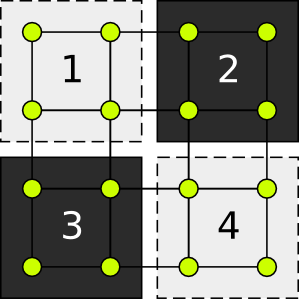
\includegraphics[width=.5\linewidth]{images/4x4.png}
  \caption{The two groups of blocks are marked with black and white squares. Here the spin orientation in block 1 and 4 can be evaluated in parallel while 2 and 3 are held still and vice-versa.}
  \label{fig:checker_grid}
\end{minipage}
\hspace{0.05\linewidth}
\begin{minipage}{.25\textwidth}
  \centering
  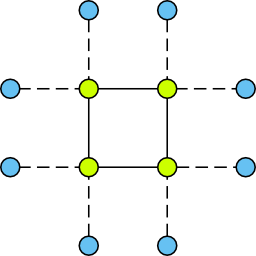
\includegraphics[width=1\linewidth]{images/2D_ghosts.png}
  \captionof{figure}{A block including its ghost cells.}
  \label{fig:gost_cells}
\end{minipage}
\end{figure}


It is further recognized that ghost cells will have to be selected with the periodic boundary condition in mind. Hence the indices of for instance the neighbouring spins in the two directions along the x-axis will be
\begin{align*}
x_+&=(x_c+1)\; \% \; L \;, \\
x_-&=(x_c-1+L) \; \% \; L \;.
\end{align*}
Here $x_+$ and $x_-$ are the indices of the neighbouring spins along the positive and negative direction of the x-axis, $x_c$ is the index of the current spin, $L$ the side of the global system and $\%$ signifies the modulus operator.

The spins will be further divided into computational threads inside each block. Theses will have access to the same shared memory and will begin to populate it with data picked from the global memory. Here, the number of spins attended to by each thread is fixed to 2. Shown for the $2\times2$ block in figure \ref{fig:2D_threads} each thread will attend to a spin at a time and to avoid race conditions a synchronization is preformed in between the two spin flips per thread. Thus the spins attended to in parallel are marked as red and green respectively for each set.
 
This division into 2 spins per thread will imply a divisibility by 2 for the block size that will in turn migrate up to the system size. Hence, the allowed system sized will be $4\times4$, $8\times8$, $16\times16$...

\begin{figure}
\centering
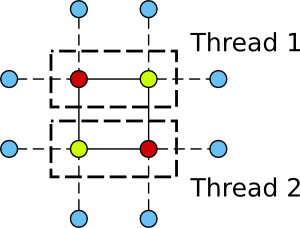
\includegraphics[width=.4\linewidth]{images/2D_threads.png}
\caption{Thread division in each block. Non-interacting spins are grouped in read and green.}
\label{fig:2D_threads}
\end{figure}

\subsection{Optimization}

\section{Results}
\label{sec:results}

\subsection{The Stiffness Exponent}

\begin{figure}
\centering
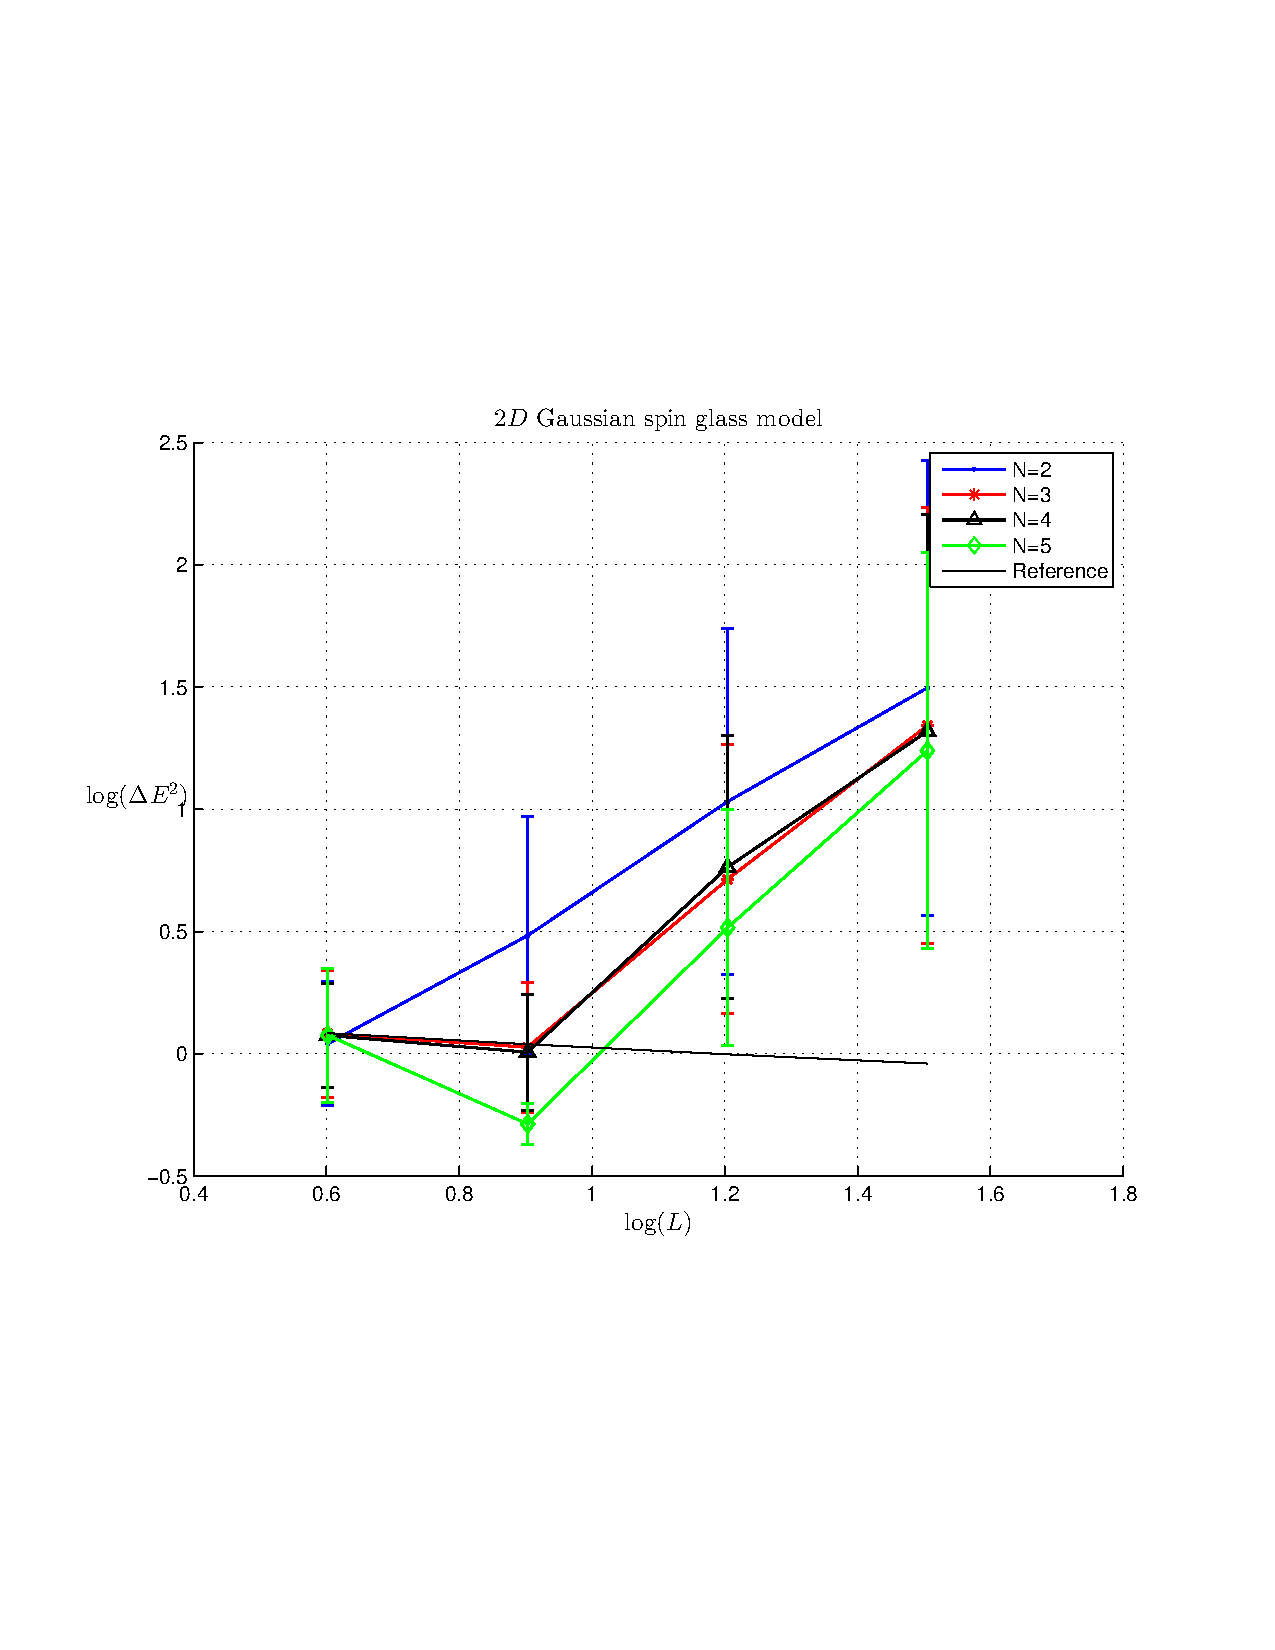
\includegraphics[width=\textwidth]{images/spinglass2D.pdf}
\caption{The square of the domain wall energy $\Delta E ^ 2$ as a function of system size $L$ for different number of quenches in two dimensions. The black line is the reference value for the stiffness exponent $\theta=-0.289$.}
\label{fig:E_2D}
\end{figure}

\begin{figure}
\centering
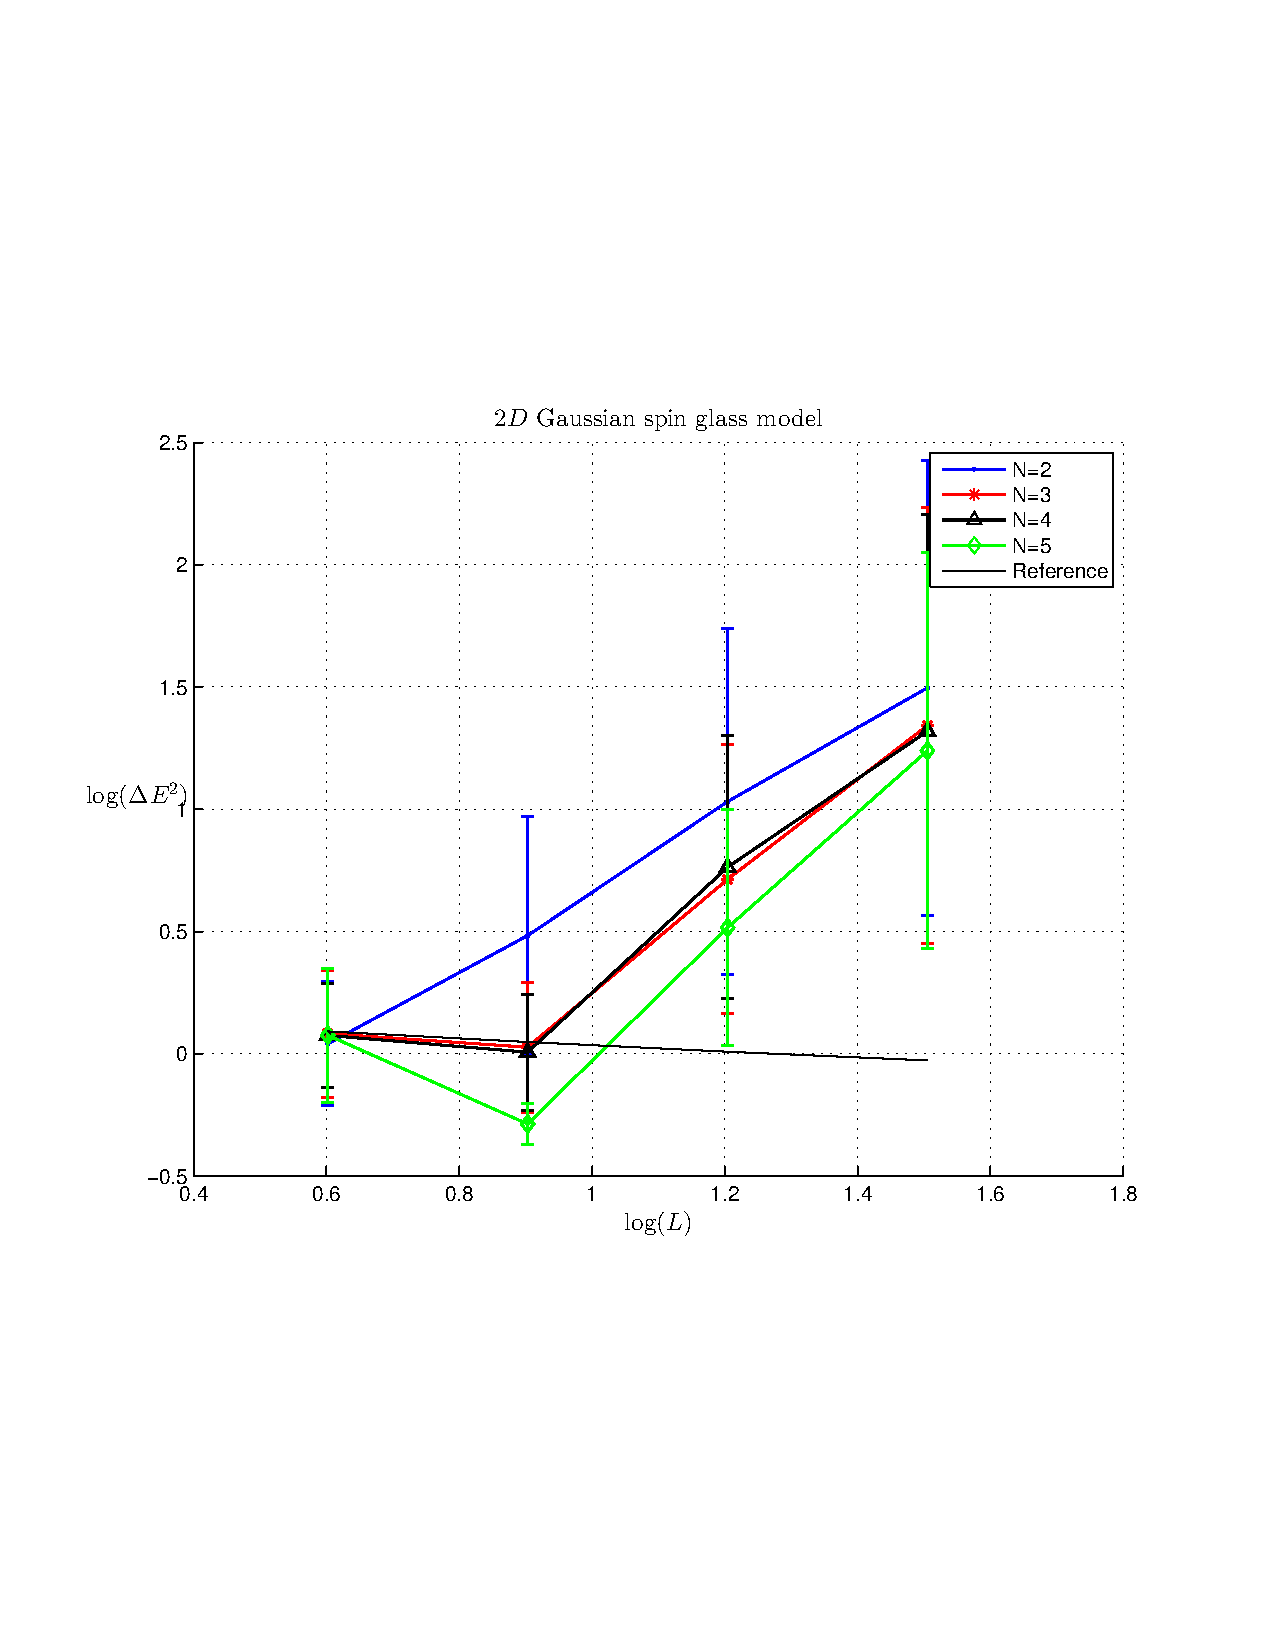
\includegraphics[width=\textwidth]{images/spinglass3D.pdf}
\caption{The square of the domain wall energy $\Delta E ^ 2$ as a function of system size $L$ for different number of quenches in three dimensions. The black line is the reference value of $\theta=0.225$.}
\label{fig:E_3D}
\end{figure}

\subsection{GPU-Algorithm Performance}

\section{Discussion}
\label{sec:discussion}
In this section we will discuss both the physical results as well as the performance of our algorithm.

\subsection{The Stiffness Exponent}
Calculating the stiffness exponent is, to say the least, a time consuming task requiring huge amounts of computations. As displayed in Fig. \ref{fig:E_2D} and \ref{fig:E_3D} the number of quenches necessary to obtain an decent approximation the ground state rapidly increases and on top of that, the time to perform each quench increases with the system size. This can be seen by observing that $(\Delta E)^2$ rapidly diverges from the expected result for a low number of quenches. This reflects the nature of the SGs with huge numbers of metastable states and the difficulty to find an approximate ground state. You need to start from increasingly many initial spin configurations in order to find a few where you do not get stuck in a local minima. The only upside with this extremely complex problem is the fact that it is parallelizable and thus well suited for computing on a GPU.

\subsection{GPU-Algorithm Performance}
[STEFAN: DISCUSSION ABOUT GPU PERFORMANCE AND BENCHMARKING TIMES]

\subsection{Concluding Remarks}
To summarize, we have calculated the stiffness exponent $\theta$ for the nearest-neighbour-interaction Gaussian Ising spin glass on a square lattice in two and three dimension using the scaling ansatz $\Delta E \thicksim L^\theta$. The domain wall energy $\Delta E$ was calculated using the P-AP method. The value for the stiffness exponent was obtained by curve fitting in a least square sense and are found to be $\theta_{2D}=-0.289$ and $\theta_{3D}=0.227$ for two and three dimensions respectively. Since $\theta_{2D}<0$ we conclude that there exists no finite temperature glass phase in two dimensions, however in three dimensions $\theta_{3D}>0$ implies that a there is indeed a finite temperature glass phase in agreement with other simulations as well as experiments\cite{hartmann}\cite{fisher}\cite{carter}. 

The implementation of the model was an optimized GPU-accelerated algorithm using CUDA which had great performance and showed great promise for future research.

\pagebreak

\begin{thebibliography}{100}

\bibitem{onsager}
Crystal Statistics I. A Two-Dimensional Model with an Order-Disorder Transition \\
L.Onsager \\
Phys. Rev. 65, 117, (1943)

\bibitem{almeida}
Chaos and stiffness exponents for short-range Gaussian Ising spin glasses \\
Sebasti\~{a}o T O Almeida, Evaldo M F Curado andFernando D Nobre \\
J. Stat. Mech (2013)

\bibitem{hartmann}
Stiffness exponent of two-dimensional Ising spin glasses for nonperiodic boundary conditions using aspect-ratio scaling \\
Phys. Rev. B 66, 224401 - Published 4 December 2002 \\
Alexander K. Hartmann, Alan J. Bray, A. C. Carter, M. A. Moore, and A. P. Young

\bibitem{fisher}
Theory of Random Magnets \\
DS Fisher, GM Grinstein, A Khurana \\
Physics Today, 1988 

\bibitem{carter}
Aspect-Ratio Scaling and The Stiffness Exponent $\theta$ for Ising Spin Glasses \\
A. C. Carter, A. J. Bray, M. A. Moore (January 4, 2014) \\
http://arxiv.org/pdf/cond-mat/0108050.pdf

\bibitem{nishimori}
Statistical Physics of Spin Glasses and Information Processing: An Introduction. \\
Nishimori, Hidetoshi (2001). \\
Oxford: Oxford University Press. p. 243. ISBN 9780198509400.

\bibitem{gpu_mc_spins}
\textit{GPU accelerated Monte Carlo simulations of lattice spin models} \\
M. Weigel, T. Yavors. \\
Physics Procedia, \textbf{15} (2011)

\end{thebibliography}
\end{document}